% !LW recipe = latexmk (xelatex)
\documentclass[UTF8,a4paper,11pt]{ctexart}
\usepackage[hmargin=24mm,vmargin=19mm]{geometry}
\usepackage{amsmath,amssymb,booktabs,graphicx,tabularx,array,xcolor}
\usepackage{float}
\definecolor{reportnavy}{HTML}{263F55}
\definecolor{reportteal}{HTML}{287F86}
\definecolor{reportcoral}{HTML}{C65D50}
\usepackage[colorlinks=true,linkcolor=black,urlcolor=reportteal,citecolor=black]{hyperref}
\setmainfont{Times New Roman}
\ctexset{section={format=\Large\bfseries\color{reportnavy}},
         subsection={format=\large\bfseries\color{reportnavy}}}
\pagestyle{plain}
\setlength{\parindent}{2em}
\setlength{\parskip}{0.10em}
\setlength{\textfloatsep}{9pt plus 3pt minus 3pt}
\setlength{\floatsep}{7pt plus 3pt minus 2pt}
\renewcommand{\arraystretch}{1.13}
\newcolumntype{Y}{>{\raggedright\arraybackslash}X}
\raggedbottom

\begin{document}
\begin{center}
{\LARGE\bfseries 可解释数据挖掘实践：RRL 在分类与回归任务中的应用\par}
\vspace{0.55em}
{\large 数据挖掘课程大作业报告\par}
\end{center}
\vspace{0.2em}

\begin{abstract}
本文完成药物诱导自身免疫预测（DIA）和鲍鱼环数预测（Abalone）两项任务，依次报告数据分析及预处理、模型训练、模型结构优化和对比分析。每项任务都比较手写线性模型、随机森林和规则表征学习器 RRL。DIA 的 597 条记录中阳性占 24.8\%，196 个数值描述符兼有稀疏、长尾和局部高度相关的特点；优化后的 RRL 在外层五折获得阳性 F1 $0.609$，高于随机森林的 $0.503$。Abalone 的 4177 条记录呈现连续尺寸趋势、强共线性和稀少的高环数样本；纯规则 RRL 的两个训练种子得到 RMSE $2.194$、$2.205$ 环，优于 Ridge 的 $2.224$ 环，随机森林仍以 $2.147$ 环领先。逐轮消融说明：DIA 的主要进步来自规则结构与训练配置的联合选择；Abalone 的连续分支虽能改善预测，却会掩盖规则自身的作用，因此最终回到纯规则主线。报告同时检查规则长度、覆盖率及导出规则与实际预测的一致性。
\end{abstract}

\setcounter{tocdepth}{1}
\tableofcontents

\section{数据分析及预处理}
\subsection{任务与分析方法}

课程任务书要求同时完成 DIA 二分类与 Abalone 回归，并从数据分析出发设计预处理和模型实验。DIA\cite{uci-dia} 合并官方训练、测试 CSV 后共有 597 条记录；原文件每行包含 \texttt{Label}、\texttt{SMILES} 和 196 个 RDKit 描述符（数据集来源网站上显示有195个Feature与实际数据有出入，以实际数据为准），本文预测 \texttt{Label}。Abalone\cite{uci-abalone} 共有 4177 条记录，以环数 \texttt{Rings} 为目标，输入为 \texttt{Sex} 与七项尺寸、重量测量值；讨论年龄时可用 $\mathrm{Rings}+1.5$，模型直接预测环数。两个数据集均无缺失值。

分析依照课堂介绍的六类工具展开。均值、中位数和众数定位数据中心，标准差及四分位距 $IQR=Q_3-Q_1$ 描述分散程度；箱线图显示中位数、四分位数和极端观测，直方图显示频数，经验分位数图显示从低到高的取值变化；散点、分箱趋势和相关系数则帮助判断变量间的关系。

\subsection{DIA：不平衡、典型分布与长尾}

先做一些简单的统计，做出图\ref{fig:dia-profile} 左侧的频数柱。DIA 的阴性 449 条、阳性 148 条，比例约为 $3:1$。这个检查很简单但是却很重要：即使始终判为阴性，也有约 75.2\% 的总体正确率，却找不到一条阳性。因此，后续保持各折类别比例，同时报告总体正确率、两类平均 F1 和阳性识别指标（因为阳性偏少，如果一视同仁对待的话，训出来的模型会天然偏向判阴性）。图\ref{fig:dia-profile} 右侧选取取值较平稳的 \texttt{MolMR} 作普通描述符参照，便于和后面的类别差异图比较。按实际观测值分类，196 个描述符中有 17 列常量、20 列严格 0/1、76 列其他整数、83 列浮点数。17 列常量不提供区分信息；主实验保留原输入维度，使原版与优化版 RRL 的比较一致。

\begin{figure}[!htbp]
\centering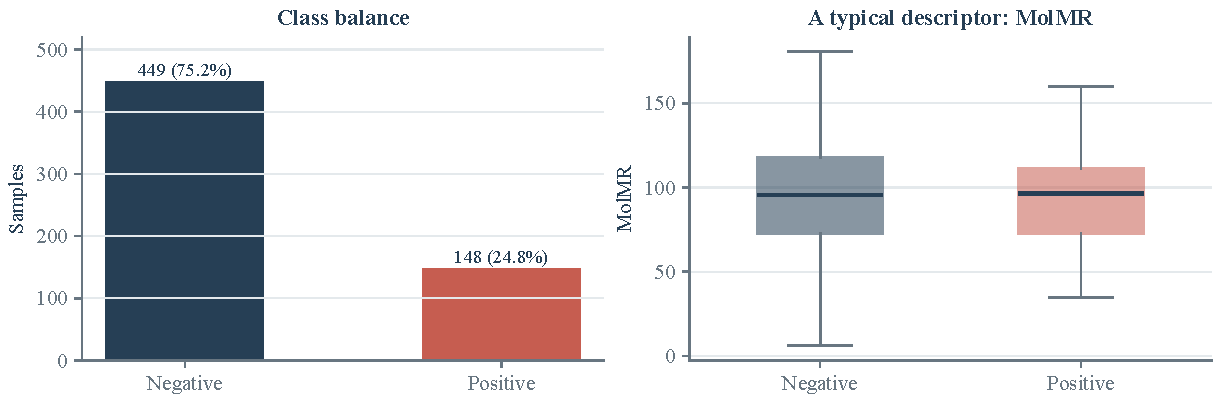
\includegraphics[width=0.83\linewidth]{figures/dia_profile.pdf}
\caption{DIA 的类别比例与普通数值描述符示例。箱体上下缘为 $Q_1,Q_3$，中线为中位数；两类 \texttt{MolMR} 的主体区域明显重叠。}
\label{fig:dia-profile}
\end{figure}

\texttt{MolMR} 的两类中位数和箱体几乎重合。箱体上下缘分别是第 25、75 百分位数，须延至 $Q_1-1.5IQR$、$Q_3+1.5IQR$ 范围内的实际观测。接着我们想知道：从单列中挑出类别差异相对明显的候选，能否只凭这一列区分阳性和阴性？先对每列计算 $D_j=|\bar x_{j,1}-\bar x_{j,0}|/s_j$，其中分子是两类均值之差，分母是该列全体样本的标准差。$D_j$ 表示两类均值相隔多少个标准差，便于比较量纲不同的描述符；它用于挑选候选，实际重叠程度还要看箱线图。图\ref{fig:dia-box} 选取取值较连续的 \texttt{FractionCSP3} 和零值较多的 \texttt{PEOE\_VSA2}，两者的 $D_j$ 分别约为 0.304、0.315，在非常量描述符中排第八、第六。它们的阴性、阳性中位数分别为 0.500/0.409 和 4.900/9.589。两类中心确实移动了，但箱体仍大幅重叠；只用单列阈值分类，容易在漏检与误报之间取舍。因此后续让规则组合多个条件，而不依赖单个描述符。

\begin{figure}[!htbp]
\centering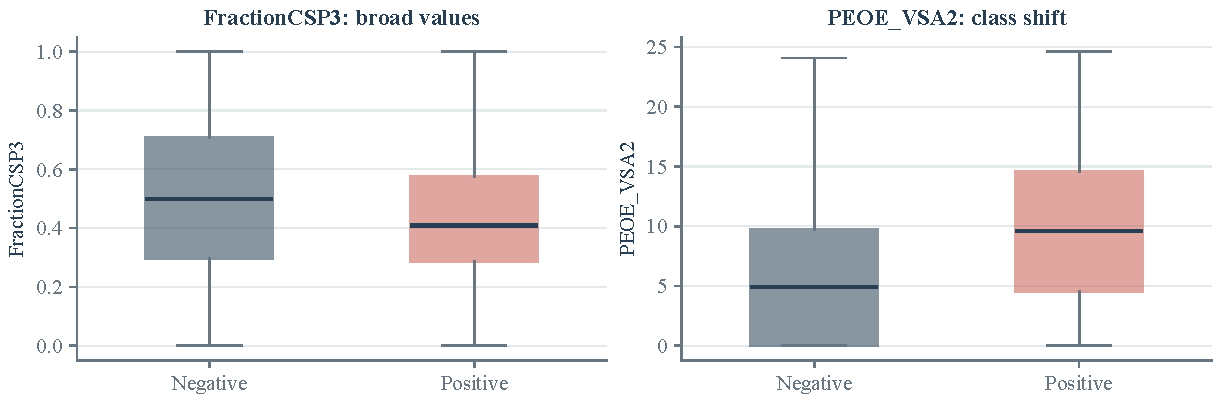
\includegraphics[width=0.81\linewidth]{figures/dia_box_comparison.pdf}
\caption{DIA 两列数值描述符的类别箱线图。\texttt{FractionCSP3} 展示较连续的常见取值，\texttt{PEOE\_VSA2} 展示更明显的类别位移；为看清箱体，图中不画离群点，统计时仍保留全部记录。}
\label{fig:dia-box}
\end{figure}

接着检查取值尺度，原因是稀疏和长尾可能让 RRL 的随机切点落在几乎没有样本的位置。58 列描述符至少 95\% 的值为零，\texttt{Ipc} 的中位数约 $4.11\times10^5$、最大值约 $3.85\times10^{14}$。图\ref{fig:dia-tail} 选这列画直方图和经验分位数：前者显示各区间的样本密度，后者不受直方图区间边界影响，便于确认上尾何时陡升。两图都显示主体集中在低值区、最高分位突然上升。直方图横轴采用 $\log_{10}$ 仅为了显示尺度，实验输入仍按各模型的训练流程处理。

\begin{figure}[H]
\centering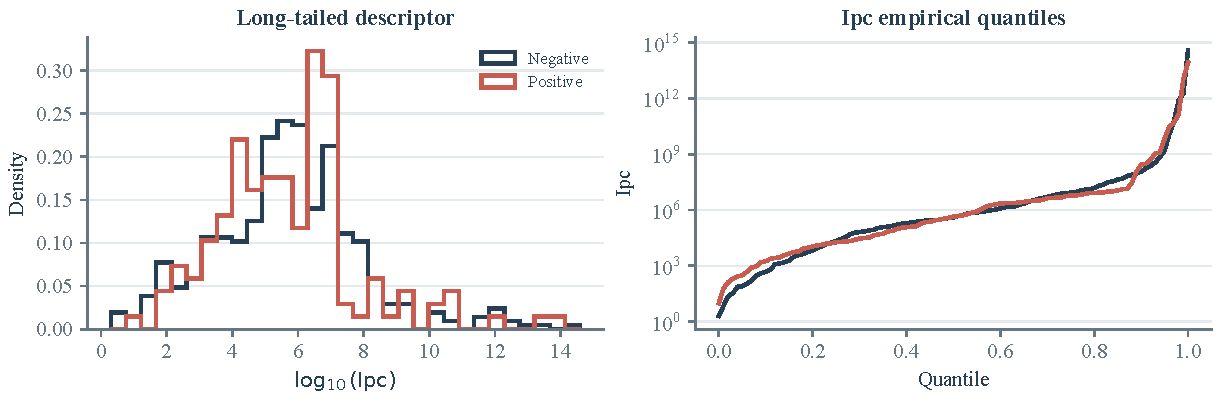
\includegraphics[width=0.83\linewidth]{figures/dia_tail.pdf}
\caption{\texttt{Ipc} 的分组直方图与分位数曲线。右图纵轴为对数刻度，尾部陡升表明少数极大值会主导原尺度的平均数。}
\label{fig:dia-tail}
\end{figure}

这样的分布启发我们检查 RRL 的切点：若随机切点落在样本稀少的区间，规则很难利用它。后续实验把当前训练集的经验分位数切点作为候选，与原始随机切点配对比较。

\subsection{DIA：单列信号与整体相关性}

最后检查两个问题：单列能提供多少线性信号，输入列之间又重复了多少信息。为此计算 Pearson 相关系数 $r$，其正负表示同向或反向变化，绝对值越接近 1，线性联系越强。179 个非常量描述符中，最大的标签相关 $|r|$ 约为 0.216；图\ref{fig:dia-corr} 右侧展示最靠前的八列，数值仍不大。这与分组箱线图的重叠相呼应。左侧把全部 $\binom{179}{2}=15931$ 对描述符的 $|r|$ 汇总：中位数为 0.068，但有 101 对达到 0.95。整体以低相关为主，局部又存在几乎重复的测量。我们保留全部描述符，让规则模型学习组合条件；删除高相关列可作为后续更精简模型的实验方向。

\begin{figure}[H]
\centering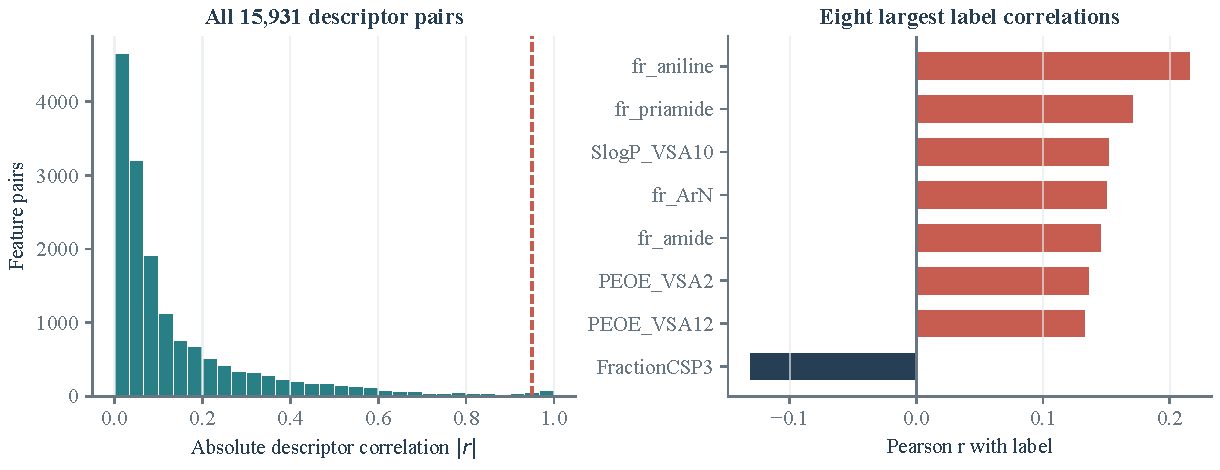
\includegraphics[width=0.90\linewidth]{figures/dia_correlations.pdf}
\caption{DIA 全部描述符对的相关强度分布，以及与标签相关性最大的八列。虚线标出 $|r|=0.95$；右图保留相关系数正负方向。}
\label{fig:dia-corr}
\end{figure}

相关系数的分布能概括全局，却看不出强相关集中在哪些列。图\ref{fig:dia-heatmap} 因此把两种尺度放在一起：左侧选标签与七列代表性描述符，保留名称和格内系数；右侧展示全部 179 列非常量描述符的 $179\times179$ 矩阵，按原始字段顺序排列，用颜色查看整体，不标密集的行列名称。右图大部分区域颜色较浅，夹杂少数较深的条带和小块；左图进一步指出 \texttt{fr\_aniline} 与 \texttt{SlogP\_VSA10} 的 $r\approx0.72$、\texttt{PEOE\_VSA2} 与 \texttt{fr\_C\_O} 的 $r\approx0.69$。标签行的系数仍较弱，支持后续尝试组合条件。

\begin{figure}[!htbp]
\centering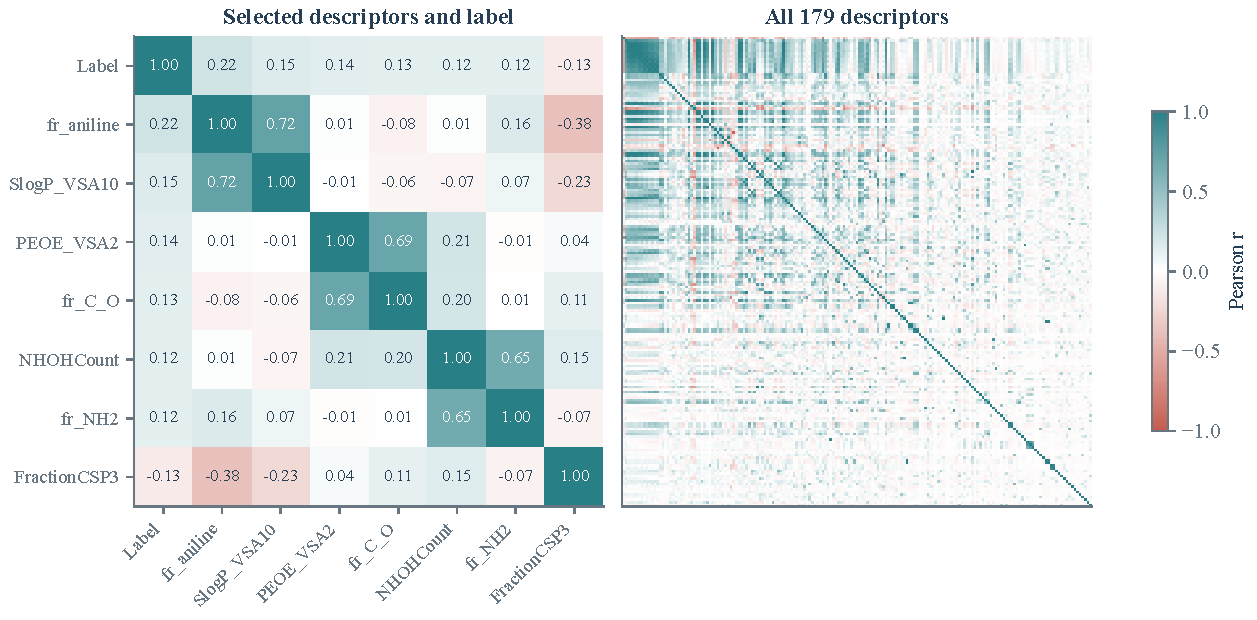
\includegraphics[width=\linewidth]{figures/dia_heatmap.pdf}
\caption{DIA 的局部与全局 Pearson 相关热力图。左：标签与七列描述符，格内标出系数；右：179 个非常量描述符的完整矩阵，不标行列名称。两图共用色标，蓝绿色为正相关、珊瑚红为负相关。}
\label{fig:dia-heatmap}
\end{figure}

\subsection{Abalone：目标、测量质量与分组结构}

先算环数的中心和离散程度，再画图\ref{fig:abalone-profile}，是为了知道模型通常要预测什么范围，以及稀少的高环数会不会被整体误差掩盖。环数的均值为 9.934、中位数和众数均为 9、标准差为 3.224；左侧直方图显示大部分样本集中在中间，$\mathrm{Rings}\ge20$ 仅 62 条（1.48\%）。右侧按 \texttt{Sex} 分组画箱线图，用同一尺度比较各组中位数和中间 50\% 的范围：F、I、M 三组平均环数分别为 11.129、7.890、10.705，I 幼体整体偏低。\texttt{Sex} 是类别而非自然顺序，输入模型时采用 One-Hot 编码；高环数则需要单独报告误差。

\begin{figure}[!htbp]
\centering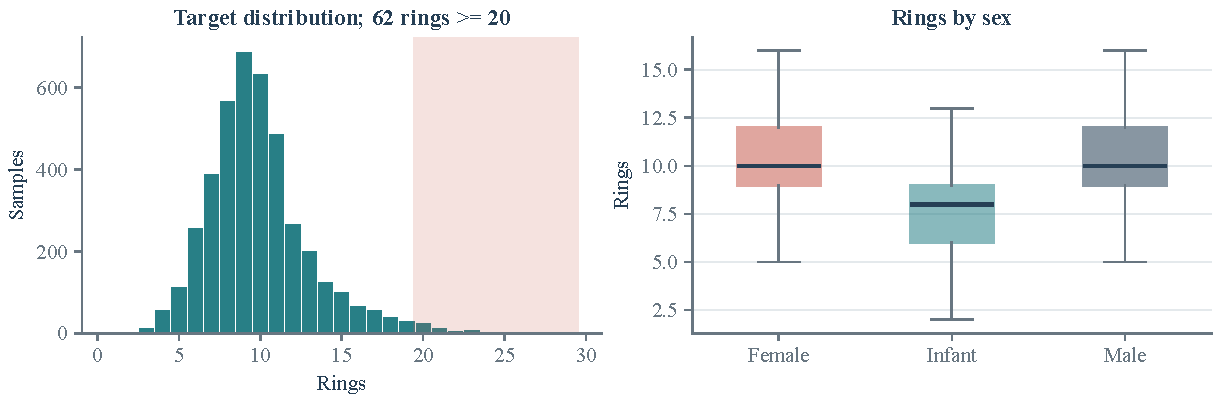
\includegraphics[width=0.83\linewidth]{figures/abalone_profile.pdf}
\caption{Abalone 环数直方图与按 \texttt{Sex} 分组的箱线图。红色浅区对应环数至少 20 的少数样本；箱体展示各组中间 50\% 的环数。}
\label{fig:abalone-profile}
\end{figure}

目标之外，还需知道七项输入通常落在什么范围、尾部有多长。表\ref{tab:abalone-measures} 因此逐列计算中位数和四分位距（表示中间一半数据的典型尺度），同时保留最小值、最大值和偏度来检查两端。偏度为正表示右侧尾巴较长，为负表示左侧尾巴较长。\texttt{Length}、\texttt{Diameter} 略向左偏，各重量字段中度右偏；\texttt{Height} 的偏度达到 3.129，与最大值 1.130 远离中位数 0.140 相吻合。数值字段的典型尺度也不同，因此线性基线的标准化参数只从训练折估计；后面再单独核查极端高度。

\begin{table}[H]
\centering\small
\caption{Abalone 七项数值输入的全数据描述统计；四分位距 $IQR=Q_3-Q_1$}
\label{tab:abalone-measures}
\begin{tabular}{@{}lrrrrr@{}}
\toprule
字段 & 最小值 & 中位数 & IQR & 最大值 & 偏度\\
\midrule
\texttt{Length} & 0.075 & 0.545 & 0.165 & 0.815 & $-0.640$\\
\texttt{Diameter} & 0.055 & 0.425 & 0.130 & 0.650 & $-0.609$\\
\texttt{Height} & 0.000 & 0.140 & 0.050 & 1.130 & 3.129\\
\texttt{Whole weight} & 0.002 & 0.800 & 0.712 & 2.826 & 0.531\\
\texttt{Shucked weight} & 0.001 & 0.336 & 0.316 & 1.488 & 0.719\\
\texttt{Viscera weight} & 0.000 & 0.171 & 0.159 & 0.760 & 0.592\\
\texttt{Shell weight} & 0.002 & 0.234 & 0.199 & 1.005 & 0.621\\
\bottomrule
\end{tabular}
\end{table}

\texttt{Sex} 三组的环数不同，也可能伴随尺寸差异。为了看清这一点，图\ref{fig:abalone-measures} 从七项输入中各选一个代表：尺寸用 \texttt{Length}，重量用 \texttt{Shell weight}，分别画分组箱线图。I 组的壳长中位数为 0.435，F、M 为 0.590、0.580；壳重中位数为 0.113，F、M 为 0.295、0.276。I 组在目标和两项测量上都偏低，说明分组信息与连续尺寸信息有关联；后续用 One-Hot 表示组别，让模型结合具体尺寸学习预测。

\begin{figure}[H]
\centering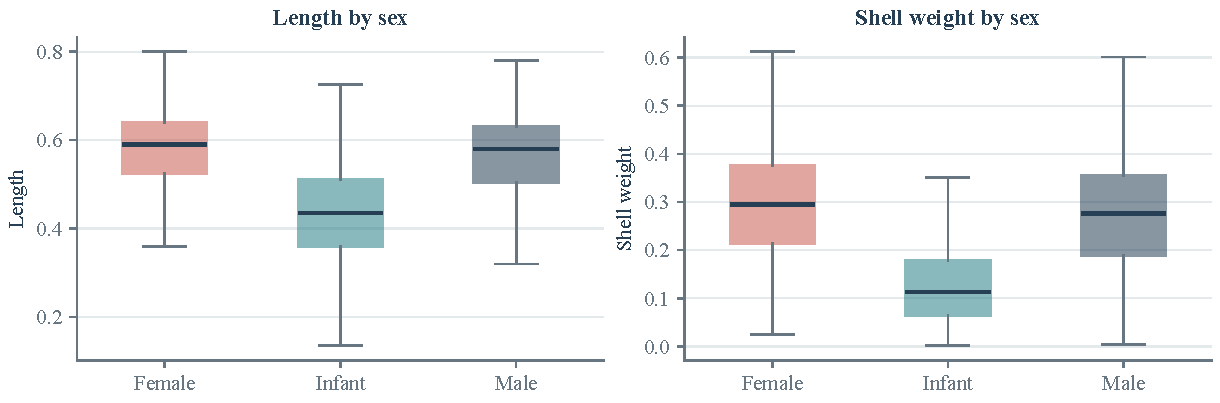
\includegraphics[width=0.83\linewidth]{figures/abalone_measurements.pdf}
\caption{Abalone 两项代表性输入按 \texttt{Sex} 分组的箱线图。左为壳长，右为壳重；箱体与须展示各组主体范围，绘图时隐藏离群点以便比较中位数。}
\label{fig:abalone-measures}
\end{figure}

直方图的形状会受分箱宽度影响，箱线图又只显示几个关键位置。为了核对完整的上尾和组间差异，图\ref{fig:abalone-quantiles} 把观测值从小到大排序，画出每个分位点的环数，以及全体高度的分位数。左图中幼体 I 的环数曲线整体低于 F、M，尤其第 95 百分位数约为 13 环，而 F、M 分别约为 17.7、17 环；这进一步说明分组差异贯穿分布，而高环数主要在尾端。右图显示 99\% 的高度不超过 0.22，最大值却达到 1.13，值得回到原始记录检查。

\begin{figure}[H]
\centering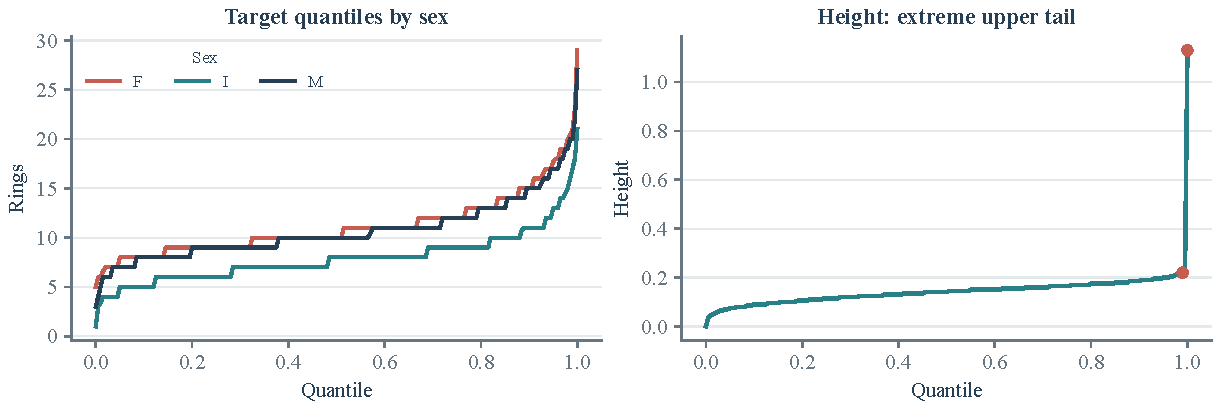
\includegraphics[width=0.83\linewidth]{figures/abalone_quantiles.pdf}
\caption{Abalone 的经验分位数曲线。左：按 \texttt{Sex} 分组的环数；右：全体高度，红点标出第 99 百分位数及最大值。}
\label{fig:abalone-quantiles}
\end{figure}

分位数指出极端值，两个测量字段的散点关系则能发现更具体的矛盾：高度应低于最长壳长，各部分重量应低于整体重量。按这些关系核查后，图\ref{fig:abalone-checks} 标出 7 条疑点：高度为零 2 条、高度大于最长壳长 1 条、去壳肉重超过整体重量 4 条；另有一条壳重超过整体重量，与高度为零的记录重合。左图红点对应高度疑点，右图红点对应肉重疑点。主实验保留原记录，并在训练折上检查剔除疑点的敏感性。按 $1.5IQR$ 标出的统计离群点数量更多，既有稀有但可信的高环数个体，也有值得复核的测量值；两者在分析中分别处理。

\begin{figure}[H]
\centering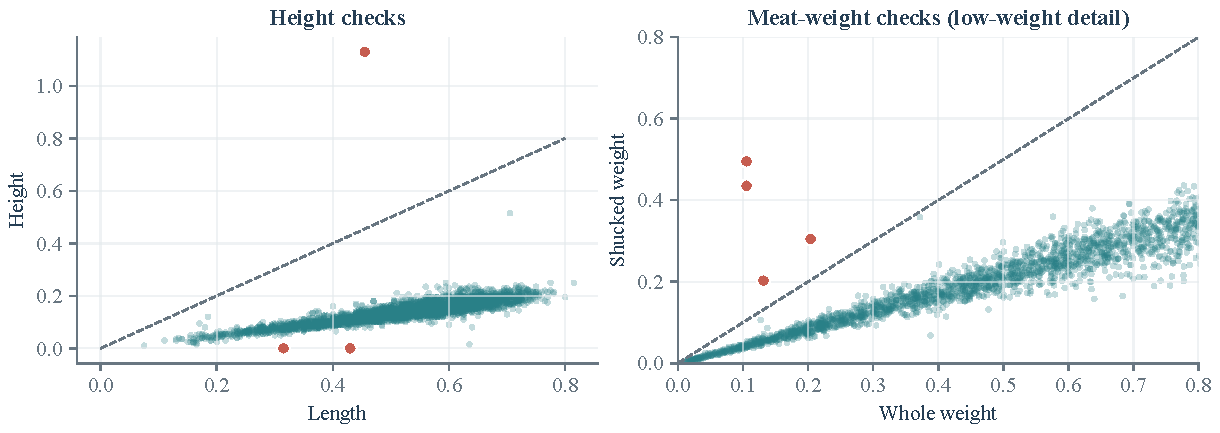
\includegraphics[width=0.82\linewidth]{figures/abalone_checks.pdf}
\caption{Abalone 测量关系与 7 条疑点。红点为不符合简单测量约束的记录，虚线表示两测量值相等；右图放大低重量区域，以便查看四条肉重大于整体重的记录。}
\label{fig:abalone-checks}
\end{figure}

\subsection{Abalone：共线性与非线性趋势}

先看单条记录而非组均值，才能知道同一重量实际对应多宽的环数范围。图\ref{fig:abalone-scatter} 因此并排画出壳重和去壳肉重对环数的原始散点，透明度较低，重叠较多的地方颜色更深。壳重与环数的上升关系较清楚，去壳肉重的点云更散；以左图阴影标出的壳重 $[0.2,0.3)$ 为例，共有 1067 条记录，环数第 10 至 90 百分位数仍从 8 跨到 14，完整范围为 6--23。重量有预测价值，但只看这一重量仍难以精确预测每条记录的环数。

\begin{figure}[H]
\centering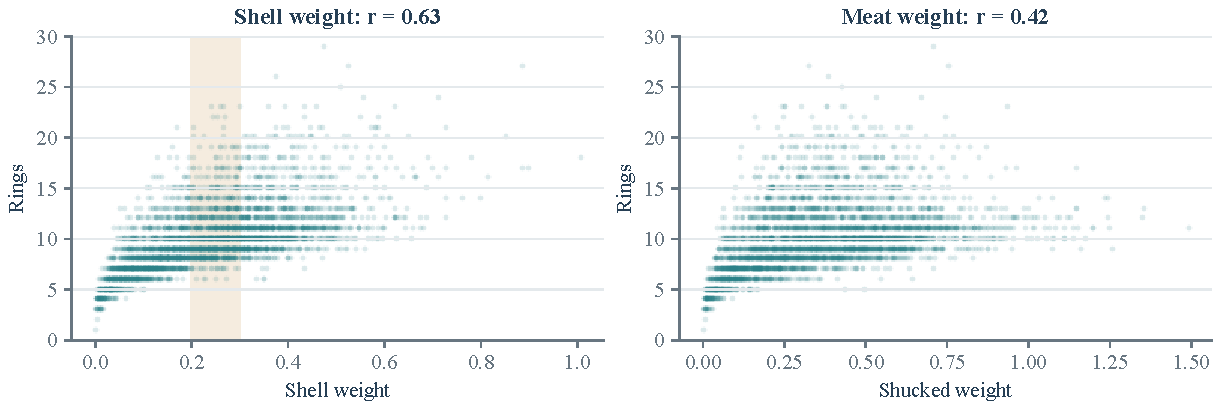
\includegraphics[width=0.83\linewidth]{figures/abalone_scatter.pdf}
\caption{Abalone 单条记录的重量与环数关系。左图阴影为壳重 $[0.2,0.3)$ 的样本带；标题中的 $r$ 为 Pearson 相关系数。}
\label{fig:abalone-scatter}
\end{figure}

散点显示样本级波动；为了汇总七项测量之间的重复信息，以及它们各自与环数的线性联系，图\ref{fig:abalone-corr} 再计算七项数值输入与环数的 $8\times8$ Pearson 相关矩阵。\texttt{Length} 与 \texttt{Diameter} 的 $r=0.987$，整体重量与去壳肉重的 $r=0.969$，两组输入存在明显共线性；环数与壳重的相关约 0.628，却与去壳肉重只有约 0.421，说明不同重量字段提供的年龄信息并不相同。强共线性会让普通线性回归的单个系数容易随样本变化，因而给线性基线加上 L2 惩罚，形成 Ridge 回归。壳重与环数的 Spearman 秩相关约 0.692，高于 Pearson 的约 0.628，提示上升趋势较明确，曲线形状还值得进一步检查。

\begin{figure}[H]
\centering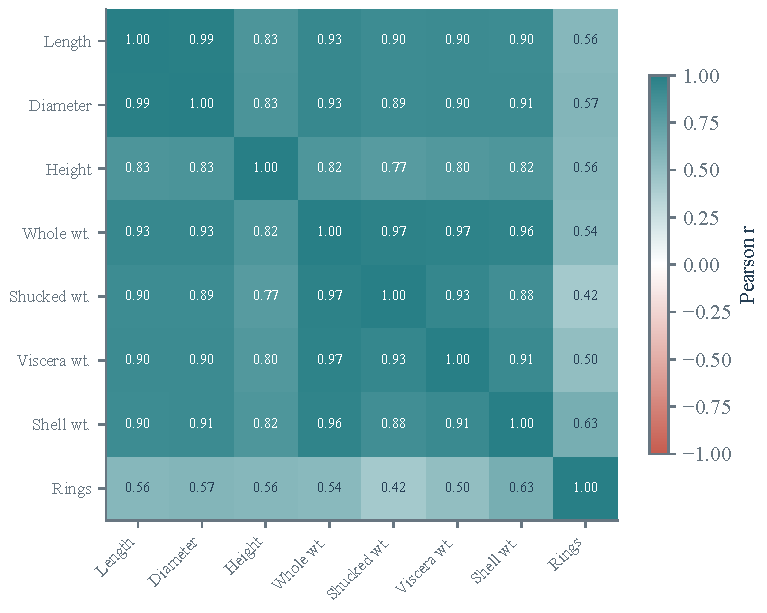
\includegraphics[width=0.66\linewidth]{figures/abalone_correlations.pdf}
\caption{Abalone 数值字段的 Pearson 相关矩阵。格内数字为相关系数；两组尺寸/重量输入之间形成明显的高相关区域。}
\label{fig:abalone-corr}
\end{figure}

原始散点显示波动范围，还需归纳曲线是否有平台。图\ref{fig:abalone-trends} 在每个 \texttt{Sex} 组内把去壳肉重、壳重各分为约八个等频箱，每个点是该箱的平均重量和平均环数。等频分箱让各点由数量相近的样本支撑，也比数千个原始散点更容易看出走向。幼体通常位于较低环数；成年组的肉重曲线后段趋缓，壳重则较稳定地上升。同一重量附近的环数仍会波动，尺寸只能解释部分年龄差异。这一观察支持把能表示阈值和交互的随机森林、RRL 与线性基线并列比较；也提醒我们纯二值规则做回归时可能损失区间内部的连续变化。

\begin{figure}[H]
\centering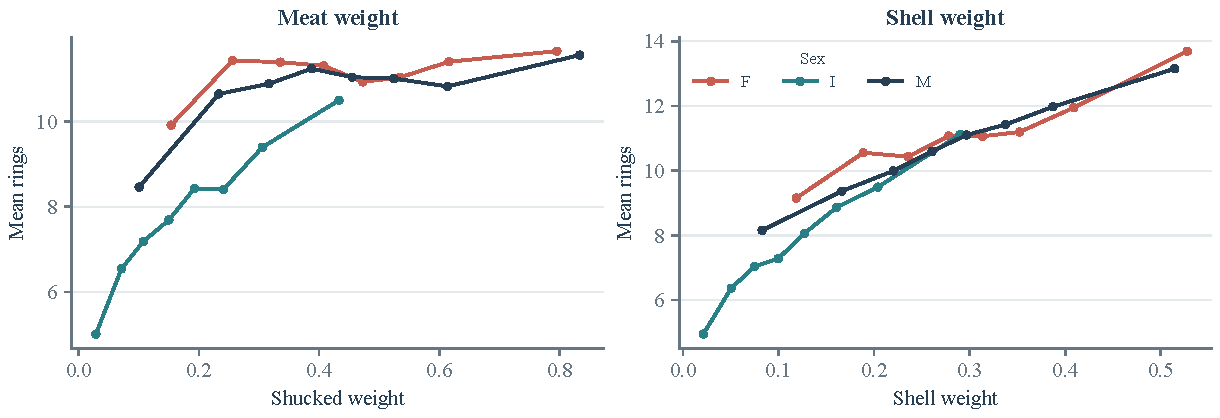
\includegraphics[width=0.83\linewidth]{figures/abalone_trends.pdf}
\caption{按 \texttt{Sex} 分组的条件分箱趋势。每条线只根据相应组的一个测量字段分箱；点为箱内平均环数。}
\label{fig:abalone-trends}
\end{figure}

\subsection{实际采用的预处理}

\begin{table}[!htbp]
\centering\small
\caption{从观察到实验处理的对应关系}
\label{tab:preprocess}
\begin{tabularx}{\linewidth}{@{}p{24mm}Y Y@{}}
\toprule
任务 & 数据观察 & 处理与验证 \\
\midrule
DIA & 阳性约四分之一 & 分层五折；报告 Accuracy、Macro-F1 与阳性 P/R/F1 \\
DIA & 零值与极长右尾共存 & 比较随机切点和训练折分位数切点 \\
DIA & 局部描述符高度相关 & 原始、优化 RRL 共用 196 列输入，保证结构实验可比 \\
Abalone & \texttt{Sex} 为无序类别 & One-Hot 编码，与七项数值测量共同输入 \\
Abalone & 数值字段尺度与尾部不同 & Ridge 在训练折内标准化；RF 使用原量纲 \\
Abalone & 尺寸/重量共线，趋势有弯曲 & Ridge 控制线性系数，RF 与 RRL 学阈值及交互 \\
Abalone & 7 条疑点、62 条高环数 & 主实验保留原始记录；做训练内敏感性及尾部误差检查 \\
\bottomrule
\end{tabularx}
\end{table}

需要标准化的输入只在当前训练子集估计均值和标准差，再把同一参数用于验证或测试子集；Abalone 的目标缩放也按此方式处理，预测时还原为环数。随机森林使用原量纲。RRL 所需的 \texttt{.data}、\texttt{.info} 文件由数据准备脚本生成。

\section{模型训练}
\subsection{三种模型如何做预测}

设一个样本的输入为 $x_i=(x_{i1},\ldots,x_{id})$，真实标签或环数为 $y_i$，样本数为 $n$。三个模型使用同一任务的同一训练/测试索引，区别在于怎样把输入映射为预测值。

\paragraph{手写线性模型。}DIA 使用逻辑回归。先计算线性分数 $z_i=w^\top x_i+b$，再经 sigmoid 得到阳性概率
\begin{equation}
p_i=P(y_i=1\mid x_i)=\sigma(z_i)=\frac{1}{1+e^{-z_i}}.
\label{eq:logistic}
\end{equation}
$w_j$ 表示第 $j$ 个标准化输入增加一个单位时，阳性对数几率 $\log[p/(1-p)]$ 的变化；$b$ 是截距。令 $y_i\in\{0,1\}$，真实类别的概率为 $p_i^{y_i}(1-p_i)^{1-y_i}$。让全部训练样本的这一概率尽量大，等价于最小化负对数似然，并给系数加 L2 惩罚：
\begin{equation}
L_{\rm log}(w,b)=-\frac1n\sum_{i=1}^n[y_i\log p_i+(1-y_i)\log(1-p_i)]
                     +\frac{\lambda}{2}\|w\|_2^2.
\label{eq:logloss}
\end{equation}
由 $\partial\sigma(z)/\partial z=\sigma(z)[1-\sigma(z)]$ 和链式法则，可得
$\nabla_wL_{\rm log}=X^\top(p-y)/n+\lambda w$、
$\partial L_{\rm log}/\partial b=\sum_i(p_i-y_i)/n$。项目中的 NumPy 实现按此梯度逐轮更新 $w,b$，预测时以 $p_i\ge0.5$ 判阳性。

Abalone 使用 Ridge 回归：$\hat y_i=w^\top x_i+b$，输出直接是预计环数。令 $\tilde X=[\mathbf1,X]$、$\beta=(b,w^\top)^\top$、$D=\mathrm{diag}(0,1,\ldots,1)$，训练目标为
\begin{equation}
L_{\rm ridge}(\beta)=\frac1n\|y-\tilde X\beta\|_2^2+\lambda\beta^\top D\beta.
\label{eq:ridge}
\end{equation}
对 $\beta$ 求导并令其为零，得到
\begin{equation}
(\tilde X^\top\tilde X+n\lambda D)\hat\beta=\tilde X^\top y.
\label{eq:normal}
\end{equation}
截距在 $D$ 中对应 0，保持不受惩罚；其余系数被适度收缩，有助于处理尺寸和重量的共线性。项目用 NumPy 求解式\eqref{eq:normal}，没有调用现成 Ridge 或逻辑回归估计器。逻辑回归与 Ridge 都给出简洁的加性预测，复杂交互则需要额外构造特征。

\paragraph{随机森林。}一棵决策树反复问“某个字段是否小于阈值”，把样本划入叶节点。DIA 树选择让子节点类别更纯的切分：若节点中阳性比例为 $q$，Gini 不纯度为
\begin{equation}
G(q)=1-q^2-(1-q)^2=2q(1-q).
\end{equation}
例如 $q=0.5$ 时两类混杂，$G=0.5$；若节点只有一种类别，$G=0$。切分成左右子节点时，选择使 $G(q)-\frac{n_L}{n_P}G(q_L)-\frac{n_R}{n_P}G(q_R)$ 最大的阈值，其中 $n_P,n_L,n_R$ 是父节点与两个子节点的样本数。Abalone 树把 $G$ 换成节点内平均平方偏差 $|S|^{-1}\sum_{i\in S}(y_i-\bar y_S)^2$，叶节点输出训练样本的平均环数。森林对训练数据有放回抽样生成多棵树，并在各切分点只考虑一部分输入字段；分类把各树的阳性概率平均，回归把各树的环数预测平均：
\begin{equation}
\hat p_{\rm RF}(x)=\frac1B\sum_{t=1}^{B}p_t(x),\qquad
\hat y_{\rm RF}(x)=\frac1B\sum_{t=1}^{B}\hat y_t(x).
\label{eq:forest}
\end{equation}
$B$ 是树的数量。不同树对样本和字段的选择有所不同，平均后预测更稳定；树还能自然组合多个阈值。实验采用 scikit-learn 的随机森林，与前述手写线性基线形成不同复杂度的参照。

\paragraph{RRL 规则表征学习器。}RRL\cite{rrl}先把输入变成真假条件，例如 $u_1=\mathbf1[\texttt{MolMR}>90]$、$u_2=\mathbf1[\texttt{TPSA}\le100]$。对每个连续阈值同时提供“大于”和“小于等于”两个条件，使逻辑层可以直接选用任一方向。逻辑层有 AND 与 OR 节点；令 $h_{kj}=\mathbf1[W_{kj}>0.5]$ 表示节点 $j$ 是否选择条件 $k$，则严格的离散输出为
\begin{equation}
R_j^{\land}(u)=\mathbf1\!\left[\sum_kh_{kj}(1-u_k)=0\right],\qquad
R_j^{\lor}(u)=\mathbf1\!\left[\sum_kh_{kj}u_k>0\right].
\label{eq:logic}
\end{equation}
前式要求所有已选条件成立，后式要求至少一个已选条件成立。多层逻辑可以把已有规则继续组合。最后的输出层把规则激活 $R_j(x)\in\{0,1\}$ 加权求和。DIA 为阴性、阳性各计算一个分数（logit）$z_c=b_c+\sum_ja_{cj}R_j(x)$，再以
\begin{equation}
P(y=c\mid x)=\frac{e^{z_c}}{e^{z_0}+e^{z_1}}
\label{eq:softmax}
\end{equation}
得到两类概率。训练时对 logits 除以可学习的正温度 $T=e^t$ 再计算交叉熵；温度改变梯度和概率尖锐程度，正值缩放保持类别排序。规则 $R_j$ 成立时，$a_{1j}-a_{0j}$ 为正表示它相对支持阳性。Abalone 把输出改为一个实数
$\hat y=b+\sum_ja_jR_j(x)$，并将损失改成 $L_{\rm MSE}=\sum_i(\hat y_i-y_i)^2/n$；例如某条规则成立且 $a_j=-0.14$，它给最终预测减少约 0.14 环。所有激活规则与截距一起决定预测，回归输出保持连续值。

式\eqref{eq:logic} 的 0/1 连接难以直接求导。RRL 的训练保留这套严格离散前向，同时用连续代理为连接参数提供更新方向。其 NLAF（新型逻辑激活函数）可写为
\begin{equation}
\mathcal G(t)=1-\frac{1}{1-(\alpha t)^\beta},\qquad
\mathcal P(s)=(1-s)^{-\gamma},
\end{equation}
\begin{equation}
\widetilde R^{\land}=\mathcal P\!\left(-\sum_k\mathcal G(1-u_k)\mathcal G(W_{kj})\right),\qquad
\widetilde R^{\lor}=1-\mathcal P\!\left(-\sum_k\mathcal G(u_k)\mathcal G(W_{kj})\right).
\label{eq:nlaf}
\end{equation}
$\alpha<1$ 保持数值有限，$\beta,\gamma$ 控制曲线形状。对 AND，每个“已选但不成立”的条件向求和项贡献违反证据；对 OR，贡献的是“已选且成立”的证据。这样把高维连乘改为加和，并可用矩阵乘法计算。梯度嫁接在前向返回严格规则值 $R$，反向采用连续代理 $\widetilde R$ 的导数，近似为
\begin{equation}
\nabla_W L\approx \frac{\partial L}{\partial R}
                    \frac{\partial\widetilde R}{\partial W}.
\label{eq:graft}
\end{equation}
输出层、逻辑连接都通过 Adam 更新，逻辑权重约束在 $[0,1]$。本项目保留原始 AND/OR、NLAF 和梯度嫁接，回归任务改动集中在输出维度与损失函数。

\subsection{五折评价、内部验证与指标}

DIA 使用随机分层五折，约每折 119--120 条，并尽量维持 24.8\% 的阳性比例；Abalone 随机打乱后分为五折，约每折 835--836 条。每轮拿一折当测试折，其余四折用于训练。以 DIA 的第二折为例，第二折暂时不参与均值、标准差、切点、超参数或早停的选择；训练完成后只在它上面评价一次。轮流换五次，每条记录恰好在一轮中成为测试样本。

训练用的四折内部还要选超参数。DIA 线性与森林基线从这四折中再留出 20\% 作验证，优化 RRL 使用内部三折；Abalone 三类模型均以内部三折选择主要参数，RRL 需要早停时从相应训练部分再留一小块验证数据。选好参数后在该轮全部四折上重新训练，再测外层测试折。内层回答“用哪套训练配置”，外层回答“这套选择流程遇到未参与选择的样本表现如何”。两任务均固定外层随机种子 0，并复用相同索引比较模型。

DIA 的阳性 Precision、Recall 和 F1 分别为
\begin{equation}
P=\frac{TP}{TP+FP},\quad R=\frac{TP}{TP+FN},\quad F1=\frac{2PR}{P+R}.
\label{eq:prf}
\end{equation}
$TP$ 是找出的真实阳性，$FP$ 是误报，$FN$ 是漏检。Precision 回答“报出的阳性有多少可信”，Recall 回答“真实阳性找回了多少”，F1 同时考虑两者。报告统一以阳性概率 0.5 为分类阈值；调整阈值会改变这三个值。

总体正确率 $\mathrm{Accuracy}=(TP+TN)/n$，其中 $TN$ 为正确判出的阴性。对阴性也按式\eqref{eq:prf} 计算一个 $F1_-$，两类取平均得到 $\mathrm{Macro\text{-}F1}=(F1_++F1_-)/2$。Accuracy 告诉我们总体判对多少，Macro-F1 让两类各占一半权重；因此表\ref{tab:dia-results} 同时列出二者和阳性 P/R/F1。ROC 与 AP 用于更完整的阈值分析，本报告主表聚焦固定阈值下的分类表现。

Abalone 用原始环数计算
\begin{equation}
\mathrm{RMSE}=\sqrt{\frac1n\sum_i(\hat y_i-y_i)^2},\qquad
\mathrm{MAE}=\frac1n\sum_i|\hat y_i-y_i|,\qquad
R^2=1-\frac{\sum_i(\hat y_i-y_i)^2}{\sum_i(y_i-\bar y)^2}.
\label{eq:regmetrics}
\end{equation}
RMSE 对大错更敏感，MAE 更接近“平均差几环”，$R^2$ 表示相对于本折直接预测均值的改善。内层按 RMSE 选参，此外单独检查环数至少 20 的样本，以观察稀少高值上的误差。

\subsection{初版训练结果}

DIA 原始 RRL 采用随机切点、\texttt{5@16} 结构（每个连续字段五个切点，每类逻辑节点各 16 个）、学习率 0.002、batch 32、训练 100 轮。手写逻辑回归比较四档 L2 强度；森林使用 300 棵树，比较三档深度与两档最小叶样本数。外层五折阳性 F1：逻辑回归 $0.465$、森林 $0.503$、原始 RRL $0.463$。原版规则能提供可执行的条件说明，但性能仍有提升空间。

Abalone 原始 RRL 同样从 \texttt{5@16} 出发，改用单实数输出与 MSE，batch 128、训练 100 轮。Ridge 搜索五档正则强度；首轮森林使用 150 棵树，比较深度与最小叶样本数。训练均值预测的 RMSE 为 $3.224$ 环，原始 RRL 为 $2.473$，Ridge 为 $2.224$，森林为 $2.147$。规则明显优于常数预测，却落后两个基线；下一节围绕 EDA 和误差现象逐轮调整。

\section{模型结构优化}
\subsection{DIA：先验证切点，再联合选择配置}

图\ref{fig:dia-tail} 显示 DIA 描述符的取值并不均匀：一些列大量为零，\texttt{Ipc} 等列还有很长的右尾。原始 RRL 随机生成切点，可能把一些切点放在样本稀少的区间。我们先只改这一处：对每个连续字段，改用当前训练子集的五个经验分位点，规则结构和训练参数保持原样：
\begin{equation}
c_{jk}=Q_{X_j}^{\rm train}(k/6),\quad k=1,\ldots,5.
\label{eq:quantcut}
\end{equation}
$c_{jk}$ 是第 $j$ 个字段从小到大排序后的第 $k/6$ 分位点；切点只由训练数据计算。原始 RRL 的阳性 Recall/F1 为 $0.418/0.463$，分位数版升至 $0.467/0.480$。这一步说明按实际分布设置切点有一定帮助，但单改切点带来的提升较小。

第二步同时考察切点、规则规模和训练方式。我们预先固定 40 套候选配置，涵盖随机、分位数和依据训练标签的 Gini 切点，以及规则宽度与深度、NLAF 参数、学习率、L2、类别权重和训练轮数等。每轮先在外层四折训练数据中再做三折验证，按验证集 PR-AUC 选出一套配置；随后用这四折重新训练，只在留出的外层测试折评价。五轮共完成 $5\times40\times3=600$ 次内部训练和 5 次外层重训，阳性 F1 达到 $0.609$，Recall 达到 $0.541$。



\subsection{Abalone：从连续分支的成功回到规则本身}

Abalone 的起点是把分类 RRL 改成实数输出和 MSE 损失，保留 AND/OR 规则，得到 RMSE $2.473$。第一轮仍只优化纯规则模型：比较 24 组切点、网络结构、损失和训练参数后，RMSE 降至 $2.290$，但仍高于手写 Ridge 的 $2.224$ 和随机森林的 $2.147$。扩大搜索也没有消除差距，于是我们开始追问：限制来自规则的训练和输出权重，还是二值条件本身丢掉了回归所需的连续变化？这一轮还核查了两个干扰因素：只在训练折移除 7 条测量疑点，收益并不稳定；分位数切点的早期优势在固定相同权重初值后缩小。因此后续比较保留原记录，并尽量配对初始化。

第二轮分别检查这两种可能。先在规则训练后固定规则，用 Ridge 重新拟合规则的输出权重；本轮纯规则对照达到 $2.257$，仍未超过 Ridge 基线。图\ref{fig:abalone-trends} 又显示重量与环数有平滑上升和局部趋缓：同一组二值条件覆盖的区间内，数值大小仍可能影响环数。我们便给输出头增加一条并行的连续通路，让原数值表示总体趋势，hinge 项 $\max(0,x-c)$ 表示切点前后斜率的变化，规则补充条件组合：
\begin{equation}
\hat y=b+\underbrace{\sum_kv_kx_k+\sum_{k,t}u_{kt}\max(0,x_k-c_{kt})}_{\text{连续分支}}
       +\underbrace{\sum_ja_jR_j(x)}_{\text{规则分支}}.
\label{eq:mixed}
\end{equation}
实现时先训练并固定 RRL 规则，再用 Ridge 联合拟合规则激活、原数值和 hinge 项的输出系数。混合模型的 RMSE 降至 $2.145$，几乎追平森林；然而用相同连续特征重新拟合、完全去掉规则后，RMSE 进一步降至 $2.124$。这一对照表明第二轮的主要收益来自连续通路，当时的规则尚未提供额外预测收益。

第三轮的目标因此变得具体：保留连续趋势的优势，同时让规则真正补充它。我们先把森林从原先 6 组扩为 72 组候选，增加树数和特征、样本采样比例等选择；扩搜后的 RMSE 约 $2.148$，与原版接近。对混合模型，我们考虑第二轮把规则系数和连续系数使用同一个 L2 强度，可能使两类信息互相牵制，于是把惩罚拆成 $\lambda_R\|a\|_2^2+\lambda_C\|v\|_2^2$：$a$ 是规则输出系数，$v$ 汇集原数值、分段线性项和类别编码的系数。规则固定后，两类系数仍用 Ridge 一起拟合。
候选还比较了固定训练轮数与训练内早停、单模型与双种子预测平均，以及先拟合连续部分再让规则学习残差。残差训练没有胜出；入选流程仍让规则直接学习 Rings，再与连续项共同预测。

第三轮混合模型的五折 RMSE 达到 $2.103$，低于扩搜森林的 $2.148$。更重要的是，保持每折相同的连续特征与惩罚设置，移除规则并重新拟合输出头后，五折 RMSE 均上升，平均高约 $0.022$ 环。规则这次在连续趋势之外产生了可测的增量；$2.103$ 对应的是分组正则、训练配置选择和双种子平均组成的混合流程。第四轮继续试局部规则斜率、更宽网络和更多成员，RMSE 为 $2.106$，没有超过第三轮。

这时需要选择报告的主线。混合模型预测更准，但式\eqref{eq:mixed} 中的连续通路承担了主要预测工作；我们希望检验仅凭学出的规则，RRL 能把回归做到什么程度。第五轮因此移除原数值和 hinge 直连，让预测重新完全由规则激活的加权和给出。沿用训练内早停，并在规则固定后只用其激活值重拟合输出权重；同时比较完整 \texttt{Sex} 编码和短规则初始化。早停的配对收益较明确，后两项没有稳定增益。相对旧纯规则对照的 $2.257$，两个种子分别达到 $2.203$、$2.205$：已经略优于 Ridge 的 $2.224$，仍落后森林的 $2.147$。

第六轮继续问如何让这些规则更短、更有信息。分位数切点覆盖取值分布，却未必最能区分不同环数；训练后的规则平均还连着约 10--11 个条件。参考逻辑网络回归与稀疏规则研究\cite{dln,ttsparse}，我们分别尝试用训练内单特征回归树确定切点，以及限制每个节点最多选择八条硬连接。表\ref{tab:factorial} 是固定配置的 $2\times2$ 对照：两项合用时，两个种子的 RMSE 小幅下降，平均条件数也降至约 7。

\begin{table}[!htbp]
\centering\small
\caption{Abalone 纯规则固定机制实验；两列种子分别训练，数字为外层五折均值}
\label{tab:factorial}
\begin{tabular}{@{}lcccc@{}}
\toprule
切点与连接方式 & RMSE 314 & RMSE 2718 & 条件数 314 & 条件数 2718\\
\midrule
分位数参照 & 2.2085 & 2.2043 & 10.47 & 11.38\\
回归树切点 & 2.1952 & 2.1969 & 11.20 & 10.43\\
连接上限 8 & 2.1984 & 2.1977 & 7.10 & 6.91\\
树切点 + 上限 8 & \textbf{2.1859} & \textbf{2.1952} & \textbf{6.92} & \textbf{7.14}\\
\bottomrule
\end{tabular}
\end{table}

固定对照中的组合策略表现较好，但完整实验仍须按训练内验证结果选模型。把 12 个候选交给内部三折和双种子评分后，外层 RMSE 分别为 $2.1942/2.2047$；全数据模型固定种子 314，选中较宽的 \texttt{20@128} 和分位数切点，未采用树切点与连接上限。因此表\ref{tab:factorial} 展示的是缩短规则的机制线索，交付模型则代表预定选参流程的结果。回看六轮：连续通路改善了混合预测，匹配消融确认规则也能补充它；回到纯规则后，模型超过简单线性基线，但与森林仍有差距。两条路线分别回答了“怎样预测得更准”和“规则本身能做到什么”。

\section{对比分析}
\subsection{DIA：少数类识别}

\begin{table}[H]
\centering
\caption{DIA 外层五折结果，阈值 0.5；均值 $\pm$ 折间标准差}
\label{tab:dia-results}
\begingroup\footnotesize\setlength{\tabcolsep}{2.5pt}
\begin{tabular}{@{}lccccc@{}}
\toprule
模型 & Accuracy $\uparrow$ & Macro-F1 $\uparrow$ & 阳性 P $\uparrow$ & 阳性 R $\uparrow$ & 阳性 F1 $\uparrow$\\
\midrule
手写逻辑回归 & $0.762\pm0.048$ & $0.656\pm0.055$ & $0.548\pm0.159$ & $0.411\pm0.060$ & $0.465\pm0.079$\\
随机森林 & $0.826\pm0.017$ & $0.699\pm0.036$ & $\mathbf{0.861\pm0.080}$ & $0.359\pm0.065$ & $0.503\pm0.063$\\
原始 RRL & $0.760\pm0.020$ & $0.654\pm0.034$ & $0.520\pm0.053$ & $0.418\pm0.065$ & $0.463\pm0.057$\\
分位数 RRL & $0.754\pm0.072$ & $0.657\pm0.056$ & $0.591\pm0.213$ & $0.467\pm0.167$ & $0.480\pm0.082$\\
联合优化 RRL & $\mathbf{0.828\pm0.029}$ & $\mathbf{0.749\pm0.041}$ & $0.696\pm0.066$ & $\mathbf{0.541\pm0.063}$ & $\mathbf{0.609\pm0.063}$\\
\bottomrule
\end{tabular}
\endgroup
\end{table}

优化 RRL 与森林的 Accuracy 约为 0.828 和 0.826，几乎持平；Macro-F1 则为 0.749 和 0.699，说明前者对两类的表现更均衡。森林报出的阳性最可信，Precision 为 0.861；优化 RRL 找回的阳性最多，Recall 为 0.541，并以 0.609 获得最高阳性 F1。这个差别很直观：森林更保守，规则模型在当前阈值下更愿意报阳性。DIA 的风险筛查更关注漏检时，RRL 的取舍较有吸引力；若误报成本高，则森林值得优先考虑。最终部署仍需按真实成本选择阈值。

\subsection{Abalone：精度与高环数误差}

\begin{table}[H]
\centering\small
\caption{Abalone 外层五折结果；误差单位为环，均值 $\pm$ 折间标准差}
\label{tab:abalone-results}
\begin{tabular}{@{}lcccc@{}}
\toprule
模型 & RMSE $\downarrow$ & MAE $\downarrow$ & $R^2\uparrow$ & $\ge20$ MAE $\downarrow$\\
\midrule
训练均值 & $3.224\pm0.122$ & $2.364\pm0.097$ & $-0.003\pm0.004$ & $11.692\pm0.684$\\
手写 Ridge & $2.224\pm0.136$ & $1.587\pm0.069$ & $0.522\pm0.038$ & $\mathbf{7.170\pm0.718}$\\
随机森林 & $\mathbf{2.147\pm0.039}$ & $\mathbf{1.514\pm0.024}$ & $\mathbf{0.554\pm0.028}$ & $7.386\pm0.632$\\
原始回归 RRL & $2.473\pm0.216$ & $1.756\pm0.148$ & $0.409\pm0.072$ & $8.960\pm1.185$\\
首轮优化 RRL & $2.290\pm0.055$ & $1.634\pm0.062$ & $0.493\pm0.015$ & $8.363\pm0.613$\\
纯规则 RRL，种子 314 & $2.194\pm0.072$ & $1.557\pm0.041$ & $0.535\pm0.015$ & $7.805\pm0.655$\\
纯规则 RRL，种子 2718 & $2.205\pm0.072$ & $1.563\pm0.049$ & $0.530\pm0.023$ & $8.000\pm0.848$\\
\bottomrule
\end{tabular}
\end{table}

纯规则 RRL 从 2.473 逐步降至约 2.20 环，两种种子都略好于普通 Ridge；森林在总体 RMSE、MAE、$R^2$ 上仍领先。图\ref{fig:abalone-scatter} 中同一重量对应较宽的环数，也解释了为什么三种模型都会留下回归误差。高环数子集呈另一种排序：Ridge 的 MAE 最低。该子集只有 62 条，五折各次测试样本更少，因此将它作为误差诊断，与总体结论并列呈现。混合连续分支曾达到 2.103，但那是另一套模型结构，表\ref{tab:abalone-results} 保留纯规则主线的可比成绩。

\subsection{规则是否真的可读、是否忠实}

线性模型的参数最少，单个系数容易查看；森林由大量树共同投票，查看某棵树只能解释整体决策的一部分。RRL 的规则直接对应模型执行的条件。比如 Abalone 最终模型中一条规则同时要求 \texttt{Length}$>0.605$、\texttt{Viscera weight}$>0.089$、\texttt{Height}$\le0.2$ 和 \texttt{Whole weight}$\le1.712$，输出权重约 $-0.141$ 环。它在训练数据上的支持度约 0.216，即约 21.6\% 的样本满足这些条件；预测还会叠加其他激活规则和截距。

规则数和长度影响阅读成本。DIA 原始 RRL 的五折平均约有 13.8 条简化规则、58.8 条硬连接；优化版约为 69.8 条规则、1806 条硬连接。更多规则提高了阳性 F1，也使整套模型难以在一页纸上读完。Abalone 最终纯规则模型有 256 个原始逻辑节点、2430 条硬连接，平均每节点 9.492 个条件；表\ref{tab:factorial} 的简化机制能进一步缩短规则，值得作为后续折中方案。

我们也核查文字规则与实际计算的一致性。DIA 保存的模型在普通前向与严格离散前向下，对五折测试样本给出相同类别。Abalone 从导出的完整规则 JSON 独立执行 NumPy 布尔计算，和保存预测的最大差约 $1.78\times10^{-15}$ 环；全数据模型重载差为零。由此，报告中的规则来自模型实际使用的逻辑结构，性能与解释可追溯到同一次实验。

\subsection{结论与复现}

DIA 的少数阳性、稀疏长尾和弱单列信号，让切点覆盖和规则组合成为关键；优化 RRL 在阳性 F1 与 Recall 上取得最好结果。Abalone 沿尺寸呈连续变化，森林总体最准确，纯规则 RRL 则在保持可执行规则的同时超过简单 Ridge。Abalone 的探索还给出两个有用的反例：额外连续分支可以显著提高分数，却需用去规则消融检查贡献；较短规则可通过树切点与连接约束得到，但最终选参未必自动偏好它。

数据下载入口是 \path{download_data.py}。统计和绘图脚本放在 \path{analysis/}，手写线性模型与 RRL 分别在 \path{models/manual_glm/}、\path{models/rrl/}；逐折预测、搜索及规则审计保存在 \path{results/dia/}、\path{results/abalone/}。本报告十二张选图由 \path{analysis/report_figures.py} 重建。\textbf{小组成员及真实分工须在正式提交前由成员填写。}

{\footnotesize
\begin{thebibliography}{9}
\setlength{\itemsep}{-1pt}
\bibitem{rrl} Z. Wang, W. Zhang, N. Liu, and J. Wang, \emph{Learning Interpretable Rules for Scalable Data Representation and Classification}, IEEE Transactions on Pattern Analysis and Machine Intelligence, 46(2):1121--1133, 2024. DOI: \href{https://doi.org/10.1109/TPAMI.2023.3328881}{10.1109/TPAMI.2023.3328881}.
\bibitem{uci-dia} X. Huang, \emph{Drug Induced Autoimmunity Prediction}, UCI Machine Learning Repository, 2025. \href{https://archive.ics.uci.edu/dataset/1104/drug_induced_autoimmunity_prediction}{UCI 1104}.
\bibitem{uci-abalone} W. Nash, T. Sellers, S. Talbot, A. Cawthorn, and W. Ford, \emph{Abalone}, UCI Machine Learning Repository, 1994. \href{https://archive.ics.uci.edu/dataset/1/abalone}{UCI 1}.
\bibitem{dln} C. Yue and N. K. Jha, \emph{Learning Interpretable Differentiable Logic Networks for Tabular Regression}, 2025. \href{https://arxiv.org/abs/2505.23615}{arXiv:2505.23615}.
\bibitem{ttsparse} H. F. Soegeng, S. K. Modi, and T. Peyrin, \emph{TT-Sparse: Learning Sparse Rule Models with Differentiable Truth Tables}, 2026. \href{https://arxiv.org/abs/2603.07606}{arXiv:2603.07606}.
\end{thebibliography}
}
\end{document}
